% !TEX root = ../main.tex

% = = = = = = = = = = = = = = = = = = = = = = = = = = = = = =
% = = = = = = = = = = = = = = = = = = = = = = = = = = = = = =

\section{Introduction}

Beginning in the 1980s, a significant amount of the cryptographic literature has been devoted to the design of e-cash systems. In the 1990s, many startups worked toward deployment of this technology but most ultimately failed~\cite{NBFMG16}. By late 2008, when Bitcoin was first proposed~\cite{Nak08}, innovation on both the academic and commercial side of digital cash had dried up. Now Bitcoin's success has breathed new life into the field: cryptocurrencies have billion dollar market capitalizations and academic conferences like \textit{Financial Cryptography} are again publishing papers on financial cryptography. 

At first glance, Bitcoin seems like a major departure from the e-cash systems from the 80s and 90s. In reality, its `academic pedigree' is a novel combination of pre-existing ideas~\cite{NaCl17}. Similarly, researchers are re-discovering long lost ideas from the e-cash literature and finding new ways to apply them in a blockchain world. For example, blinded coins were a staple of e-cash~\cite{Cha82} that re-emerge, along with accumulators~\cite{SaTa99}, in post-Bitcoin systems like zcash~\cite{MGGR13,SCG+14}. Enabling micropayments through lottery-based probablistic payments of macropayments was explored in the 90s~\cite{Riv97,Whe97,JaOd97} and re-emerged for Bitcoin~\cite{Pash15}. In this paper, we `re-discover' the 1997 payment system \pw from Rivest and Shamir~\cite{RS96}. 

\pw is a credit-based payment system, envisioned for small payments. The mechanics we will turn to later, but for now, the reader can think of tokens being issued that have some value. The key limitation of \pw is that tokens do not have inherent value; their value is based on the trust assumption that a counter-party will honour the value ascribed to them. With Ethereum and other blockchain technologies, we can fix this issue by stapling cryptocurrency to the token through the use of a smart contract. Finally, while Ethereum already has internal functionality for payments, \ew enables payments to be made off-blockchain and settled once on-blockchain.

This transformation turns \pw from a trust-based credit system to a escrow-based payment system; not unlike offline payment channels and networks being proposed for Bitcoin --- the Lightning Network being the most prominent~\cite{PD15}. After presenting our system, \ew, we discuss its relation to payment channels (see Section~\ref{sec:pcn}). It is known that an Ethereum-based payment channel will be less complex than a Bitcoin one, since most of the complexity of Bitcoin-based payments channels (\eg \textblue{setup is XX transactions and payment is YY}~\cite{MMSH16}) comes from Bitcoin's limited scripting language. \ew a uni-directional (monotonic) payment channel that can be chained into a payment network and has very compact (\eg 256-bit) payments. It thus might be an interesting primitive to enhance in the same ways other payment channels~\cite{DW15,PD15} have been: adding features~\cite{KG17}, increasing efficiency~\cite{DEFM17,MBKM17}, and adding transactional privacy~\cite{GM17,MMK+17,HAB+17,RMKG18}.

% = = = = = = = = = = = = = = = = = = = = = = = = = = = = = =
% = = = = = = = = = = = = = = = = = = = = = = = = = = = = = =

\section{Preliminaries}

\subsubsection{Hash Chains}

A hash chain~\cite{Lam81} is constructed by iteratively applying a public one-way hash function $\Hash{}$ on a random value $s$. Let the notation $\HashN{i+1}{s} = \Hash{\HashN{i}{s}}$. A hash chain of length $n+1$ is:
\begin{equation*} \tuple{s,\Hash{s},\HashN{2}{s},\HashN{3}{s},\ldots,\HashN{n-1}{s},\HashN{n}{s}} \end{equation*}

where $s$ (technically equivalent to $\HashN{0}{s}$) is called the \textit{seed} and $\HashN{n}{s}$ is called the \textit{tip}. Given the hash is preimage resistant against a computationally bounded adversary, knowing some value in the chain $\HashN{x}{s}$ does not reveal any values `up' the chain from it, including the seed: $\tuple{s,\ldots,\HashN{x-1}{s}}$. Conversely the value $\HashN{x}{s}$ can be iteratively hashed to produce the rest of the values `down' the chain ending up producing the tip value. 

\subsubsection{Recognition}

 If Alice meets Bob at a party, Bob can give the tip of a chain to Alice as a token~\cite{ABC+98}. Later when Bob meets Alice again, he can provide $\HashN{n-1}{s}$ as proof he is the the same person that gave her the token. On the subsequent visit, he provides $\HashN{n-2}{s}$ and so on for $n$ visits. Of course, Bob could more directly provide Alice with his public key and sign messages each visit, however hash chains avoid the relatively expensive public key operations of a signature scheme.

\subsubsection{Payments}

In \pw, recognition is used for credit-based payments. A customer generates a length $n+1$ hash chain and provides a signed tip to the merchant. They agree that each preceding value in the hash chain has a specified unit of value owed to the merchant by the customer. For example, say $n$ is 100 and the value of each hash in the chain is a \$1 debt owed to the merchant. To expense \$27, the customer provides $\HashN{n-27}{s}$ to the merchant who will verify that hashing it 27 times produces the signed tip. The customer can increase the amount by sending further hashes, up to \$100 (after which, the payment channel is \textit{exhausted} and must be reinitiated).

% = = = = = = = = = = = = = = = = = = = = = = = = = = = = = =
% = = = = = = = = = = = = = = = = = = = = = = = = = = = = = =

\section{\ew}

\ew is a succinct Ethereum-based smart contract written in Solidity (see Appendix~\ref{sec:code}). The primary issue with \pw is that payments have no actual value and only represent an agreement to pay. In \ew, we staple Ethereum's internal currency ether (ETH) to the payments through a smart contract to give them real value. Thus \ew eliminates the counter-party risk in accepting payments that is inherent in \pw, and this is only possible because payments are backed by both a digital currency and a decentralized execution environment. We follow the standard paradigm used in the literature to eliminate counterparty risk (sometimes called claim-or-refund~\cite{BK14}). If Bob (the sender) wants to send up to $X$ \eth to Alice (the receiver), he prepays by loading $X$ \eth into a smart contract that the receiver can withdraw from when specified conditions are met. The sender also sets a deadline for the receiver to withdraw, after which he can release the escrowed funds back to himself. The receiver checks that the contract is properly formed and funded; only then will she accept payments from the sender.

\subsection{Code Design}

\begin{Protocol*}[t!]
\begin{framed}
\textbf{Title}\\
\footnotesize

\textblue{
\begin{compactlistn}
\item Construct
\item Open
\item Check
\item Receive
\item Close
\end{compactlistn}
}
\normalsize	
\end{framed}
\caption{Caption and stuff\label{alg:lab}}
\end{Protocol*}

\textblue{\ew is designed with two main functions that mediate the transaction process between $C$ and $M$. First, the contract is instantiated by $C$ through calling the \texttt{open} function. In this function, $C$ initializes the contract through passing the pseudonym of the merchant's account $M$, the tip of the hash chain $\_root$ so that the contract can verify released intermediate hash values against it, the amount that each released hash value is worth $\_wordvalue$, and the total amount of the whole hash chain $\_balance$, and $T_{end}$ which is the time after which remaining funds in the contact's balance are refunded to the customer's account. After calling the \texttt{open} function, both the contract and merchant can evaluate the length of the chain and, thus, $M$ can offline know how many intermediate hash values she can accept from $C$ without the need to constantly monitor the state of the contract. Also, $M$ knows that she has to claim aggregated payments before $T_{end}$ or else, $M$ can refund the contract's available balance.For each payment in the form of an intermediate hash $x=h^i(s)$, $i=1,2,\cdots,N-1$ that $M$ receives from $C$, she can verify its validity offline by evaluating if $h^{(N-i)}(x) = h^N(s)$ or not. Accordingly, $M$ can decide whether to accept the transaction or decline it in the event of a failed verification. After a few micropayments, where $M$ has acquired a set of intermediate hashes, she invokes the \texttt{claim} function in the smart contract by passing to it the last received hash value $wordScratch$, and its order within the hash chain $n$. Consequently, the contract verifies the validity and the required balance of the supplied inputs against the stored hash chain parameters, and upon successful verification, the account of $M$ is credited by the resulting balance.}

\subsection{Relation to Payment Channels}
\label{sec:pcn}

\textblue{Payment channels were proposed as a . Monotonic. Unidirectional. Fixed Capacity. }

\subsection{Forming payment networks} 

\textblue{Consider three parties: the cash-provider, the cash-taker, and an intermediary. To funnel a payment through the intermediary, both the cash-provider and the the intermediary set up a contract with the same tip (wordValue). They make one modification, claim is made a public function. Done.}

\subsection{Porting to Bitcoin}

\textblue{\pw almost works in Bitcoin script. Transactions can be hash-locked and scripting supports iterative scripting. The issue is that the number of hashes to invoke cannot be a parameter of inputScript.}


% = = = = = = = = = = = = = = = = = = = = = = = = = = = = = =
% = = = = = = = = = = = = = = = = = = = = = = = = = = = = = =


% = = = = = = = = = = = = = = = = = = = = = = = = = = = = = =
% = = = = = = = = = = = = = = = = = = = = = = = = = = = = = =

\section{Evaluation}

\subsubsection{Footprint}

\begin{table}[t]          
\centering
\begin{tabular}{ l | r | r }
System 		& SLOC 	& Payment Size 	  \\ \hline
\textsf{Pay50} 	& 37  	& 264 bits  		  \\
\eww 		& 31		& 776 bits  		  \\ 
\end{tabular}
\caption{Footprint in terms of code complexity and size of offline payments between \eww and \textsf{Pay50}. We modernized \textsf{Pay50} slightly, both implementations comply with linter SolHint; simple lines of code (SLOC) is per GitHub's metric.\label{table:loc}}
\end{table}

A recent blog post by Di Ferrante argues for the simplicity of Ethereum-based payment channels (relative to Bitcoin) and he offers a `50 lines of code' Solidity implementation of a uni-directional, monotonic channel we will name \textsf{Pay50} for the purposes of this paper~\cite{DF17}. As a barebones implementation, it is simple but it relies on offline payments to be signed by the sender. We deploy a lightweight version of \ew that strips out some of the functionality (\eg more flexible funding) and security protections (\eg the state machine) of the code in Appendix~\ref{sec:code}. This version, called \eww, is a line-by-line replication of \textsf{Pay50}, substituting in \ew functionality as relevant. As seen in Figure~\ref{table:loc}, \eww does not add to the lines of code; in fact, it even shaves a few off. The more important property is the size of the payment sent to the receiver; this is reduced from a digital signature to a hash or from 776 bits to 264 bits. Note that it is even possible to reduce \eww to 256-bits; an extra 8 bit value representing the length of the hash from the tip is included for a more convenient loop.

\subsubsection{Gas Costs}

\begin{table}[t]          
\centering
\begin{tabular}{ l | r | r | r }
Function & Gas & ETH & USD \\ \hline
Constructor 		&317\,299  	& 0.0067 	& \$5.88 \\
Open 			&12\,129 		& 0.0002 	& \$0.22 \\ 
Claim (50) 		&21\,511  	& 0.0005 	& \$0.40 \\
Claim (100) 		&25\,772  	& 0.0005 	& \$0.48 \\ 
\end{tabular}
\caption{Cost of running the basic contract functions. Since claim is dependent on how long the hash chain is for the claimed payment, the function shows costs for length 50 and length 100. See Figure~\ref{fig:gas} for more on this.\label{table:gas}}
\end{table}

\begin{figure}[t]
\centering
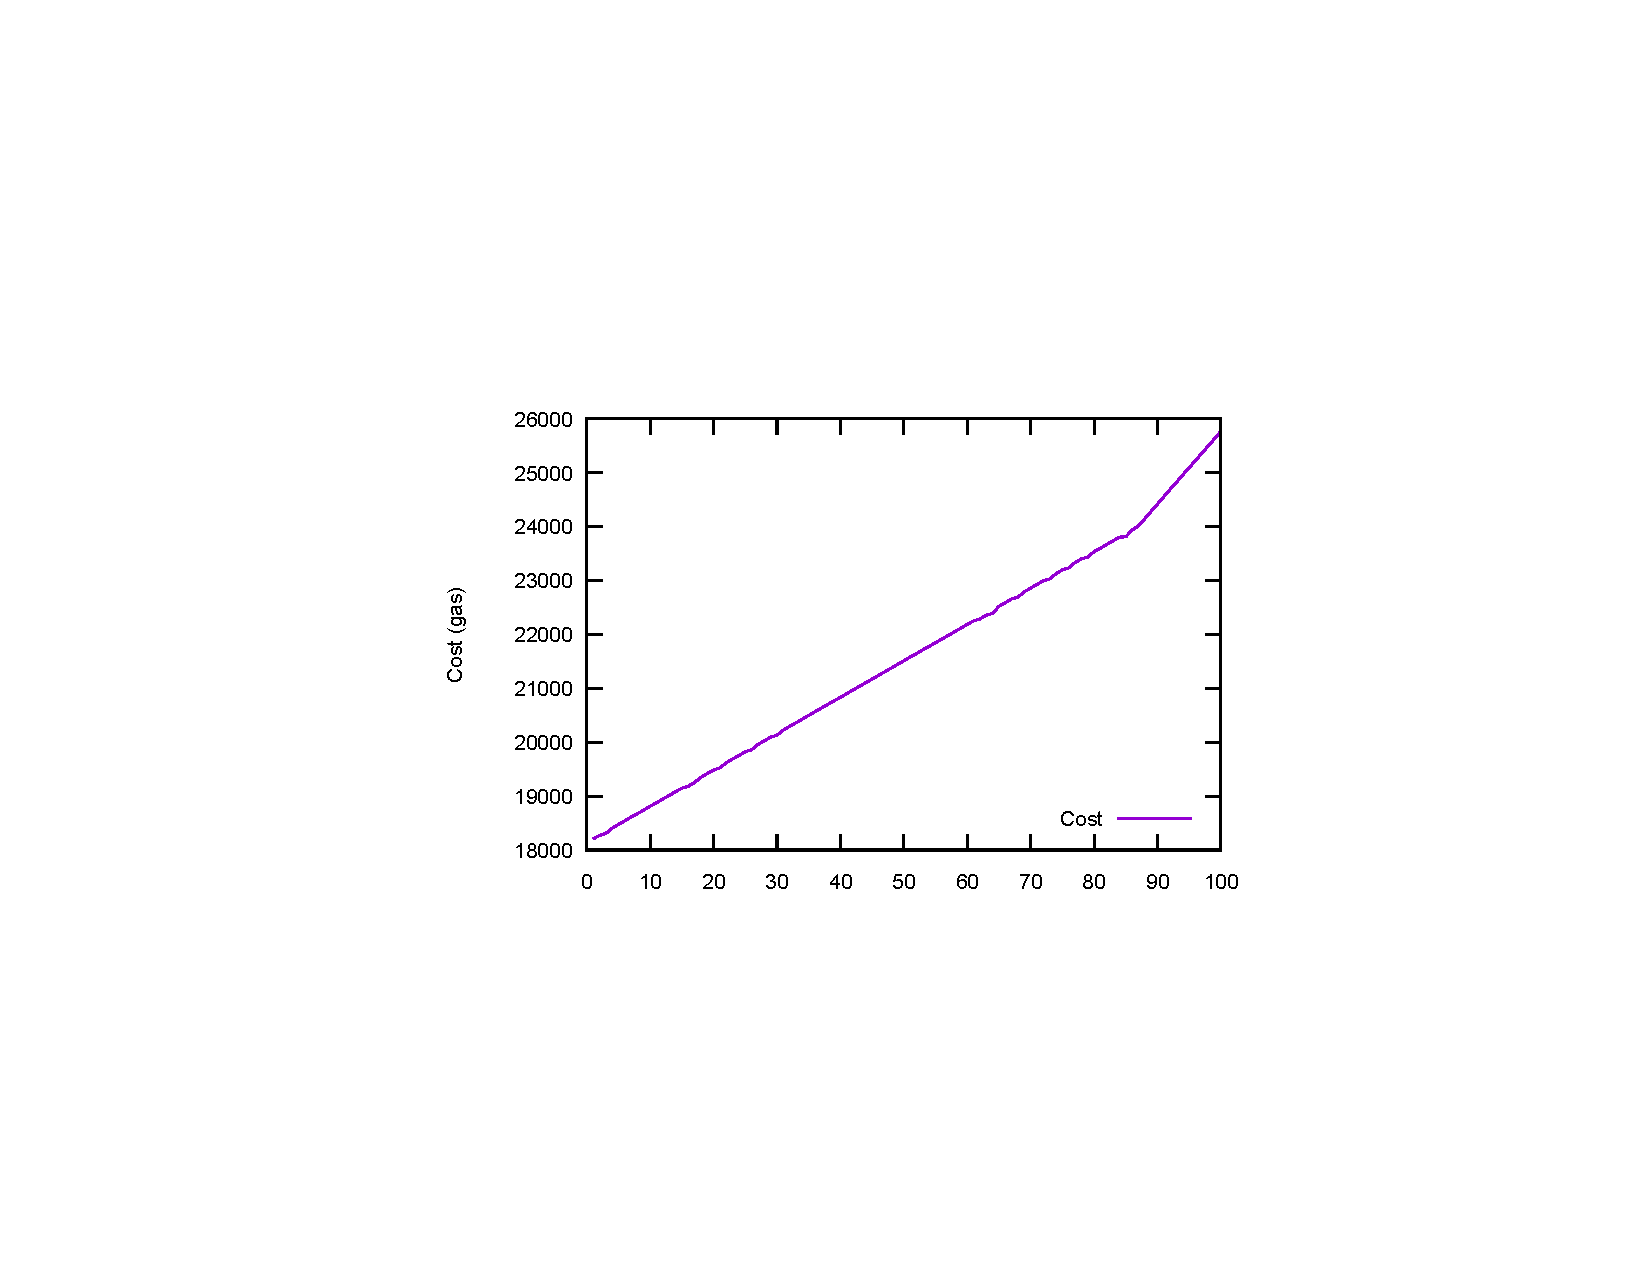
\includegraphics[width=\linewidth]{figures/gas.pdf}
\caption{The gas cost of the claim function as a function of the length of the hash chain. The gas cost of a claim in \textsf{Pay50} is around \textblue{42\,000}.\label{fig:gas}}
\end{figure}

As of January 2018, the price of 1 gas is $21\times10^{-9}$~ETH\footnote{https://ethstats.net/} and the exchange rate of 1 ETH to USD is \$882.92.\footnote{https://coinmarketcap.com/} We show the gas costs of each function in \ew if run successfully. The cost of the claim function includes checking if the provided payment (hash) is part of the hash chain (if when iteratively hashed, it results in the tip value). Thus the cost of claiming will vary on how many times the hash must be iterated. For example, consider a channel with 100 payment values worth \$1 each. Running claim on the payment value representing \$5 will require hashing the value 5 times. The payment value of \$95 will require 95 hashes and thus cost more. 

In Figure~\ref{fig:gas}, we show the gas cost of the claim function as the number as the length of the chain varies from 1 to 100. At 100, the cost is 25\,772 which is still about half the cost of running a claim function that must verify a digital signature (\eg \textsf{Pay50} uses the \texttt{ecrecover} operation in Solidity with some additional processing logic).

\subsubsection{Contract Security}

\textblue{Reentry, state machines, static analysis, time dependence, tod}

%\subsubsection{Security Properties}
%
%EthWord smart contract provides the following guaranteed security properties:
%\begin{itemize}
%	\item Fair exchange of services:
%	\item Conducting irrefutable transactions without blockchain monitoring:
%\end{itemize}

% = = = = = = = = = = = = = = = = = = = = = = = = = = = = = =
% = = = = = = = = = = = = = = = = = = = = = = = = = = = = = =

\section{Discussion}

\subsection{Use cases and limitations} 

\textblue{Prepay is dumb, at \$5 it isn't really micropayments}

\subsection{Trickling} 

\textblue{Resolve fair exchange by trickling payments}













